
\chapter {\noun{Data Flows}}
In this section we present diagrams that are needed to describe part of the system.
\section{\noun{Use Cases}}
\begin{figure}[h]
\centering
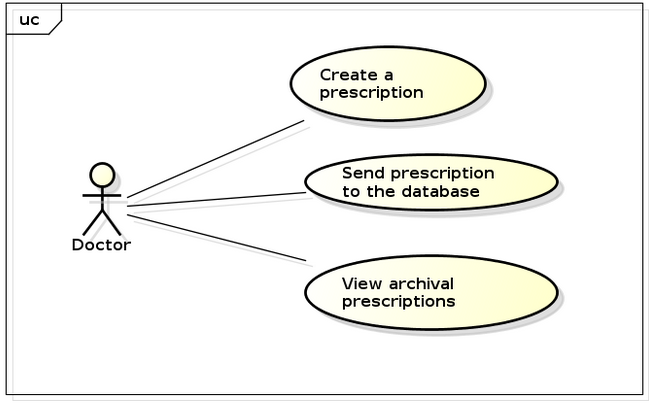
\includegraphics[width=1\textwidth]{doctor/UseCases.png}
\end{figure} 
We mark out 3 use cases:

\begin{itemize}


\item \textbf{create a prescription} - Doctor is generating prescription by collect all needed data and then signature is forged
\item \textbf{send prescription to the database} - prescription sending to database( in some database friendly format)
\item \textbf{view archival prescriptions} - Doctor can check archival prescription of his current patient
\end{itemize}

\section{\noun{Activity diagram}}
It presents system scheme from high level layer and has to show the overall flow of control
\begin{figure}[h]
\centering
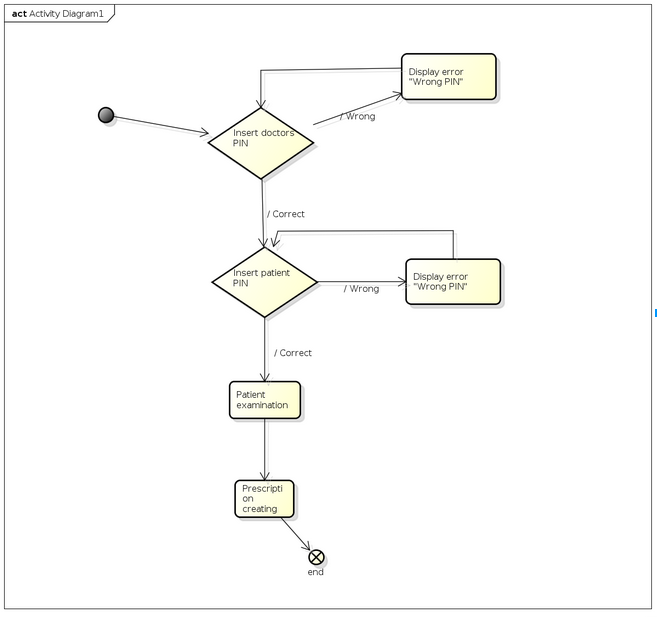
\includegraphics[width=0.8\textwidth]{doctor/ActivityDiagram.png}
\end{figure} 

\chapter{\noun{Sequence Diagram}}
We present detailed scheme of the system. THe mail goal of this diagram is to present communication between out part, and other parts of the system

\begin{figure}[h]
\centering
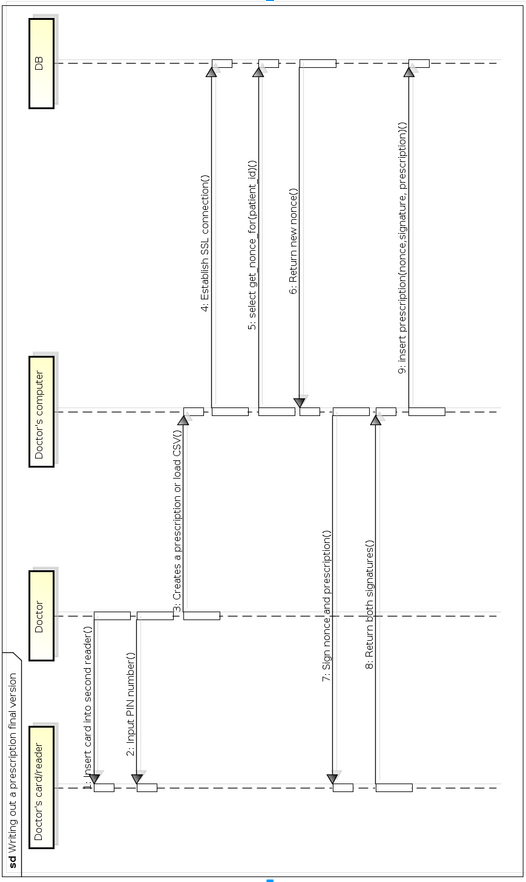
\includegraphics[width=\textwidth]{doctor/WritingOutPrescription.png}
\end{figure} 


Writing out a prescription is initialized by the doctor. He can create a prescription on demand or load one previously saved from the csv file. During creation process patients ID should be obtained (from reading patients card or returned by database query). Having newly created prescription, Doctors computer is establishing SSL connection to the database. After this stage, computer requests new value of nonce, by the SQL statement  \texttt{getnoncefor(patientid)}.  This nonce and entire prescription should be signed be the doctors card. At the end of the process query to database is made. It should include: nonce, signature over nonce, prescription and signature over prescription.

Database validates both signatures and nonce before inserting any records. Only information inside database can be considered as valid.
%%//Added to there
\section{\noun{View Entire Patient's History}}

\begin{figure}[h]
\centering
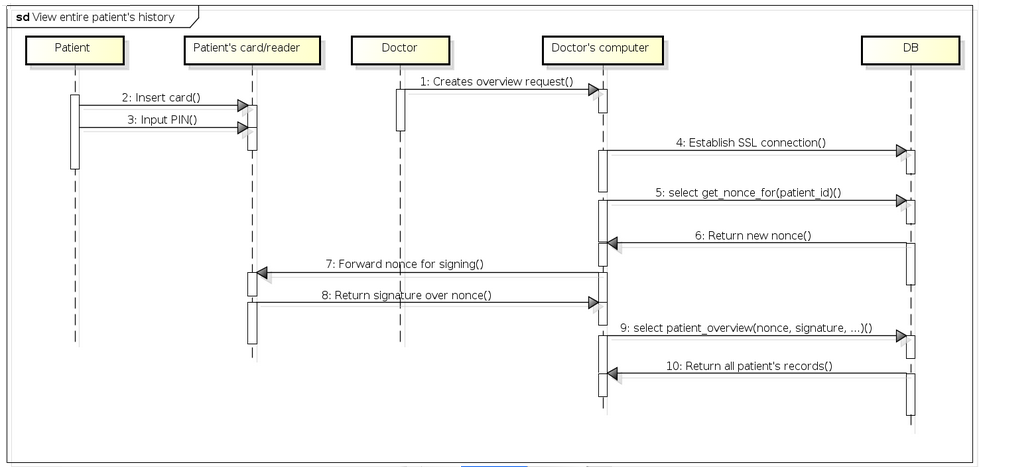
\includegraphics[width=\textwidth]{doctor/HistoryCheckout.png}
\end{figure} 

View entire patient`s history is initialized by the doctor. First of all, doctor creates overview request. During the process patient`s ID should be obtained(from reading patient`s card or returned by database query). Having the request, Doctor`s computer is establishing SSL connection to the database. After this stage, computer requests new value of nonce, by the SQL statement  \texttt{getnoncefor(patientid)}.  This nonce and entire prescription should be signed be the doctor`s card.

At the end of the process query to database is made. It should include: nonce, signature over nonce, request and signature over request.  Database after successful  validation return patient`s records.


\section {\noun{Notes}}
There is no need to require doctor's signature in this procedure. Process requires the presence of a patient and his willingness, so only the owner of the card should be verified. Adding doctor`s signature doesn`t change anything. It only increase computation time and data amount sended across the internet. 

\chapter {\noun{Prescription}}
In this part we propose structure of prescription defined using ASN.1. We do not specify format of records in database, it is just a formal specification of object \texttt{ Prescription} with information that it has to contain(i.e. it can be even concatenation of all fields specified lower splited by \texttt{;}).

\begin{figure}[h]
\centering
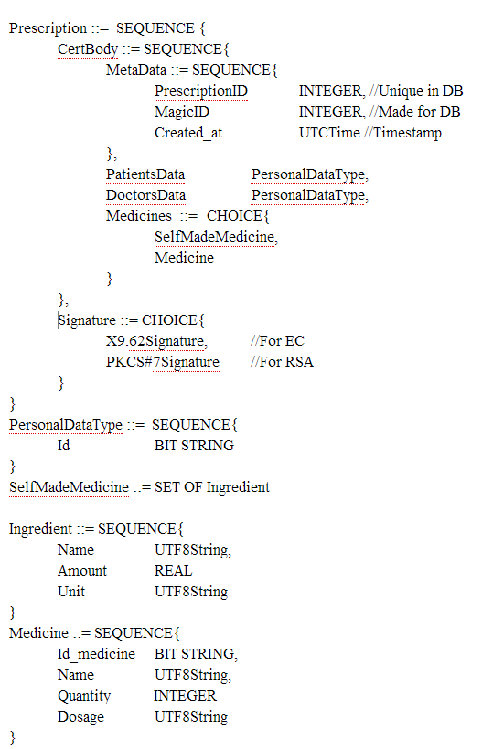
\includegraphics[width=\textwidth,height=\textheight,keepaspectratio]{doctor/asn1.png}
\end{figure} 
In this model it is obvious that pharmacist`s signature is equal to fully realized prescription


\chapter {\noun{Signatures}}
There is a lot of signature schemes that can be used according to standards (like PKCS\# or X9.63) so we do not specify which should be used yet. We want to mark a situations in protocols that has to be signed.
\section{\noun{Doctor signature over prescription, and pharmacist signature as a proof that prescription is realized}
}
Prescription as a tuple of data and signature can be signed by doctor and then creating prescription process has been completed. Now when pharmacist is realizing prescription, he has to generate another signature over that tuple with some pharmacist personal data and concat it to prescription. If pharmacist sign prescription, it means that prescription is realized (fully because there is only 1 medicine per prescription)

In this scenario there is still possibility to generate prescription without patient knowledge, but it can not be realized without him, so this scheme is still secure. 

Doctor has to compute signature, because it is a proof that prescription is valid and is signed by specified person. Without it, there is possibility to craft a lot of prescription without knowledge who is trying to spam database.

\section {\noun{Patient needs to generate signature when patient archival prescription has to be available}}

There is a use case, when a doctor wants to look into archival prescription of a patient. Core of a system sends then a nounce (random generated byte`s array) that has to be signed by a patient as a proof that patient allow doctor to check his archival prescription. The Core is not signing a nounce so there is possibility to Adversary (i.e. doctor) to make chosen message attack, so we need to choose digital signature scheme that is unbreakable by chosen-message attack(should we specify what is this?). 

Patient needs to generate signature because he is computing a request that says to DB that he want access to archival prescription. Without it, we do not have a mechanism to confirm this request by patient, so there is opportunity to make request for access without a patient knowledge.


